\subsection{Trackpy}
\label{sec:link2d:trackpy}

The \texttt{link} function from the Trackpy~\cite{trackpy} library is able to perform the \link* task both in 2D and in 3D.

Originally, it required the located positions to be inside a \texttt{Pandas Dataframe}, and it used to convert it into a \texttt{NumPy} array.
However, since our data was already inside a \texttt{NumPy} array with the same format, the library was altered to avoid this useless conversion, thus saving time.

\subsubsection{Algorithm}

The Trackpy library implements the Crocker-Grier linking algorithm~\cite{trackpy-link}.

\subsubsection{Evaluation}

For a single camera, the linking speed was 40 FPS.
If different cameras were analyzed in parallel processes, 3 cameras could be processed at an overall speed of 120 FPS.

The quality was good at a visual inspection (see figure~\ref{fig:linkDD:trackpy} or the full video~\cite{linkDD-trackpy}), and the total number of tracklets was around 6500.

\begin{figure}
	\centerline{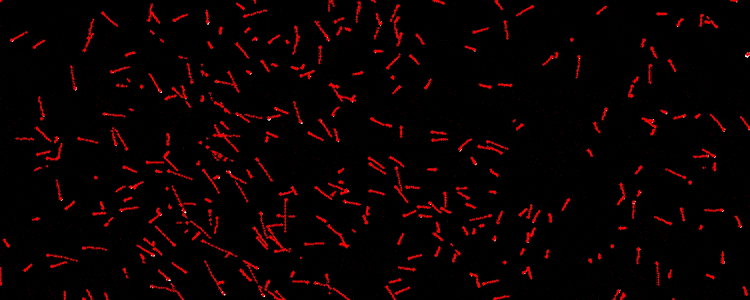
\includegraphics[width=\locateimgsize]{images/link2d/trackpy.png}}
	\caption{\centering A frame from the Trackpy \linkDD* result, full video available at~\cite{linkDD-trackpy}}
	\label{fig:linkDD:trackpy}
\end{figure}
